\documentclass[anchorcolor=blue,linkcolor=blue]{beamer}
\usepackage{booktabs}
\usepackage{amsmath}
\usepackage{xcolor}

\definecolor{links}{HTML}{07568E}
\hypersetup{colorlinks,linkcolor=,urlcolor=links}

%%\usepackage{blkarray}
\mode<presentation>
{
%  \usetheme{Malmoe}
\usetheme{default}
%\usecolortheme{seahorse}
  % or ...

 \setbeamercovered{transparent}
  % or whatever (possibly just delete it)
 \setbeamertemplate{footline}[default]
 \setbeamertemplate{navigation symbols}{\insertslidenavigationsymbol\insertframenavigationsymbol\insertdocnavigationsymbol}
}
\usepackage[english]{babel}

\title{\huge What can your library do for you?}
\author{Rajarshi Guha, Dac-Trung Nguyen, Ajit Jadhav\\
NIH NCATS\\ \vskip 2em \textit{ACS Fall Meeting 2016, Philadelphia}}

\begin{document}

\begin{frame}
  \titlepage
\end{frame}

\begin{frame}
  \frametitle{Library Design}
  \begin{itemize}
  \item Historical collections and assay data provide information on how a set of compounds has faired
  \item Use (dis)similarity and machine learning to construct new collections that show similar behavior
    \begin{itemize}
    \item Plus various constraints
    \end{itemize}
  \item If sufficiently annotated, compound behavior can be correlated to assay and biology characteristics
  \end{itemize}
\end{frame}

\begin{frame}
  \frametitle{Two Questions}
  How likely are compounds, associated with a  given annotation, identified as active?
  \vskip 2em
  Given a new set of compounds, what sets of assay conditions (as implied by the annotations) will they be active in? 
\end{frame}

\begin{frame}
  \frametitle{Prior Work}
  \begin{itemize}
  \item BAO annotated datasets
    \begin{itemize}
    \item \href{http://www.ncbi.nlm.nih.gov/pubmed/24441647}{de Souza et al, 2014}; \href{http://www.ncbi.nlm.nih.gov/pubmed/23155465}{Vempati et al, 2012}
    \end{itemize}
  \item Analyzing HTS datasets using BAO
    \begin{itemize}
    \item \href{http://www.ncbi.nlm.nih.gov/pubmed/25512330}{Zander-Balderud et al, 2015}; \href{http://www.ncbi.nlm.nih.gov/pubmed/21471461}{Sch\"{u}rer et al, 2011}
    \end{itemize}
  \item Semi-automated annotation of assay descriptions using the BAO 
    \begin{itemize}
    \item \href{http://www.ncbi.nlm.nih.gov/pubmed/25165633}{Clark et al, 2014}
    \end{itemize}
  \end{itemize}
\end{frame}

\begin{frame}
  \frametitle{BAO 2.0}
  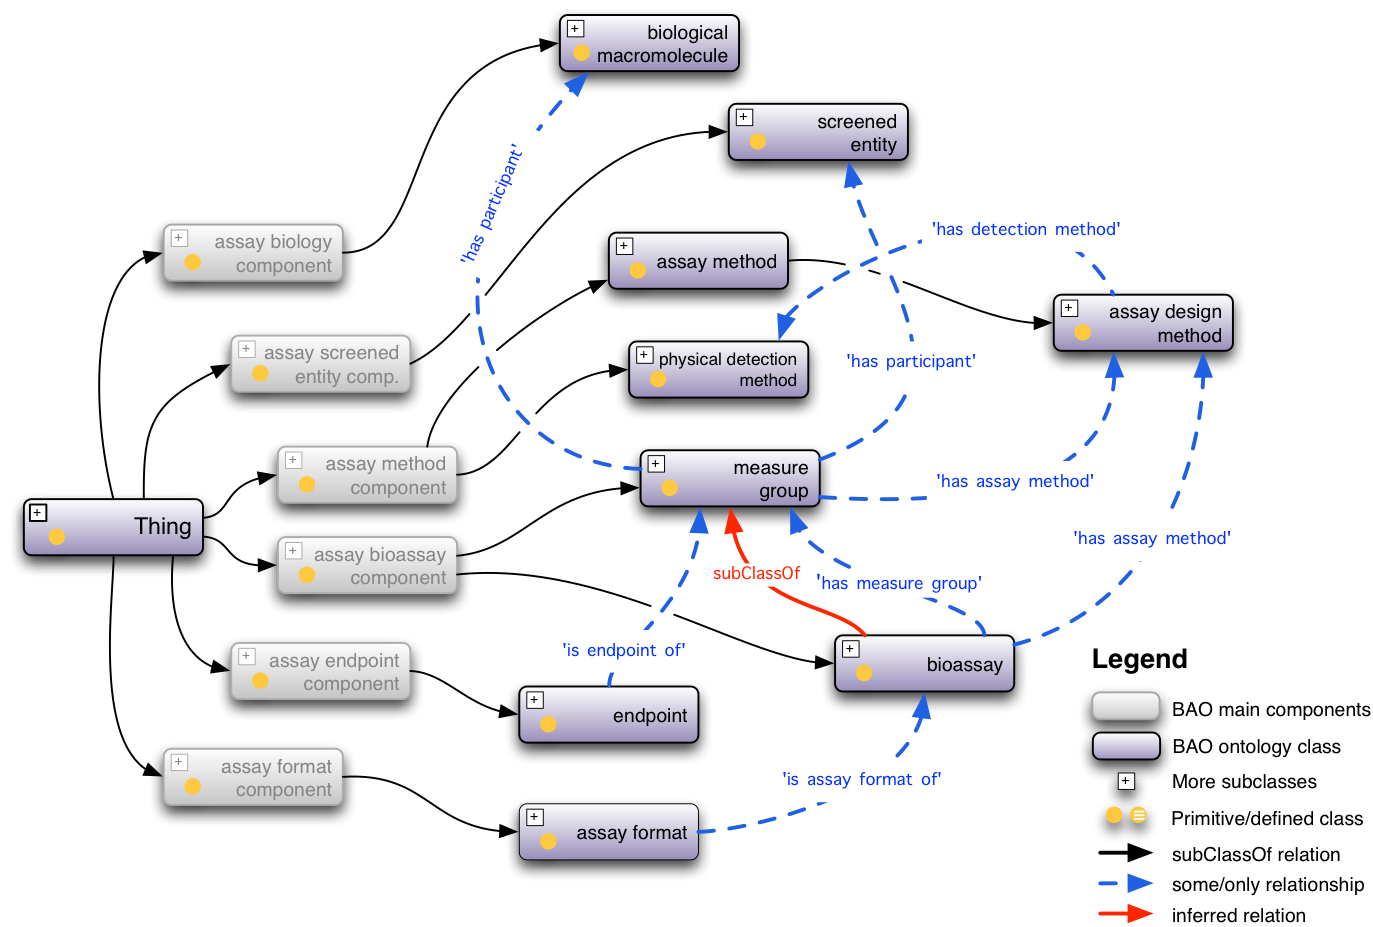
\includegraphics[height=3.0in]{bao}
\end{frame}

\begin{frame}
  \frametitle{Assay Modeling}
  \begin{center}
    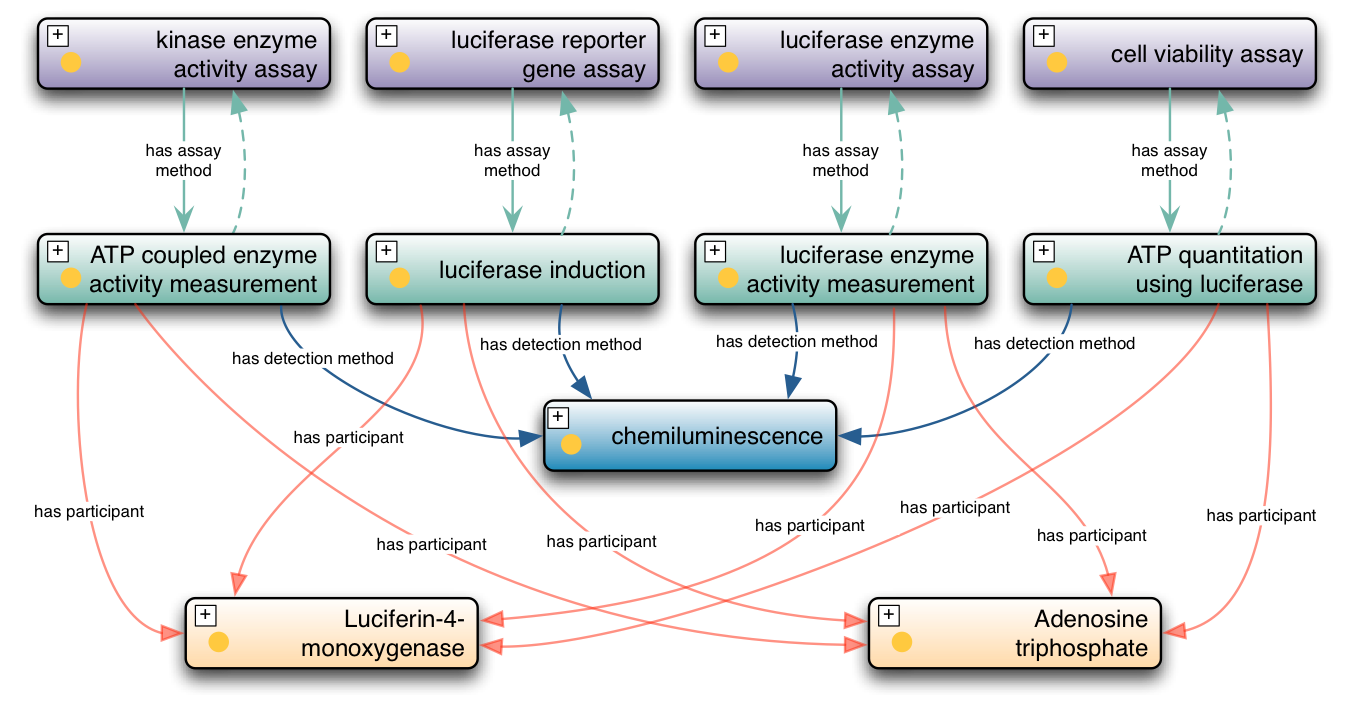
\includegraphics[width=0.9\paperwidth]{assaymodel}    
  \end{center}
\end{frame}

\begin{frame}
  \frametitle{Workflow}
  \begin{itemize}
  \item Extract unique BAO terms and for each term identify annotated assays
  \item Extract active compounds from this set of assays
  \item Compute fingerprint bit distribution
  \item Use these conditional bit distributions to identify the BAO terms that describe the assay that they are likely to be active in
  \end{itemize}
\end{frame}

\begin{frame}
  \frametitle{Dataset Overview}
  \begin{itemize}
  \item Extracted 4010 Pubchem AIDs from BARD
  \item Primary, confirmation, counterscreening assays
  \item 154M outcomes
  \item 740K compounds
  \item 192 unique BAO terms
  \end{itemize}
\end{frame}

\begin{frame}
  \frametitle{Dataset Overview}
  \begin{center}
  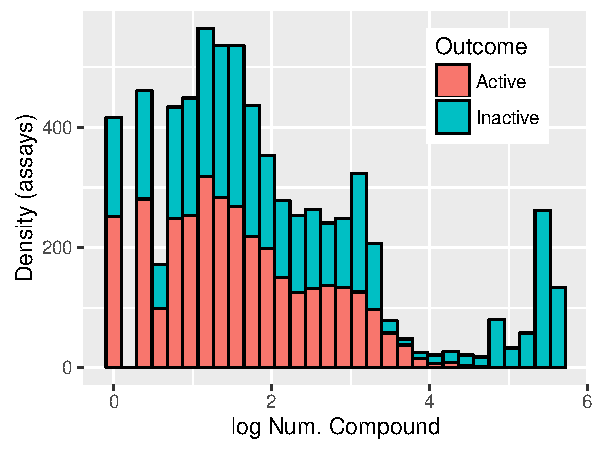
\includegraphics[width=0.5\textwidth]{img-outcomehistogram}
  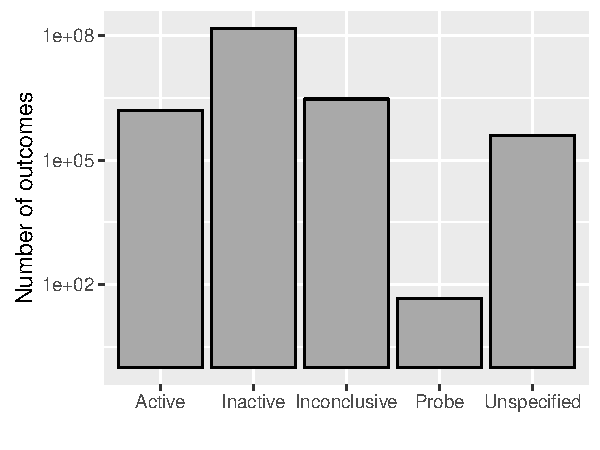
\includegraphics[width=0.5\textwidth]{img-bioassay-outcomes} \\
  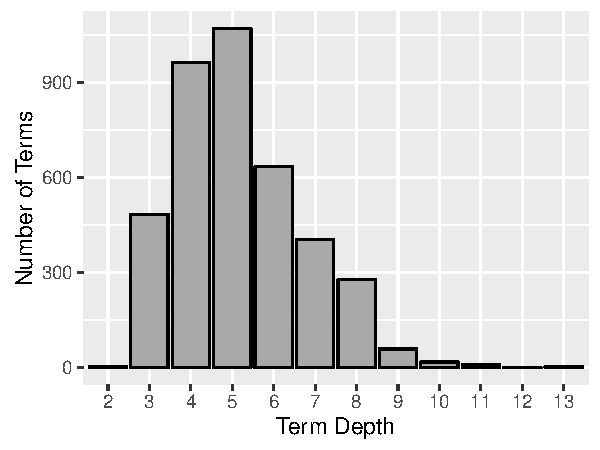
\includegraphics[width=0.5\textwidth]{img-termdepth}
  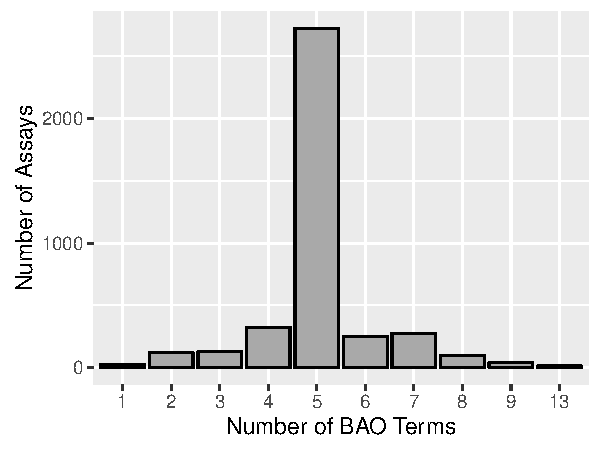
\includegraphics[width=0.5\textwidth]{img-termassaycount} \\    
  \end{center}
\end{frame}

%%%% per-term NB model
% \begin{frame}
%   \frametitle{Per-Term Na\"{i}ve Bayes Models}
%   \begin{itemize}
%   \item Predict liklihood of being active, given an ontology term
%     $T_i$ and given a set of  features $\{B\}$  
%   \item Model this using Na\"{i}ve Bayes in which the two classes are
%     $T_i$ and ``Other''
%   \item Results in a set of models $\{M_1, M_2, \cdots, M_N\}$ where $N$
%     is the number of unique ontology terms. \vskip 1em
%   \item For a new compound in library, obtain probability of term $T_i$ using
%     model $M_i$
%   \item Aggregate top $k$ terms from each model for each compound in
%     the library and select top $n$ terms
%   \item \textbf{Represents the set of ontology terms defining an assay in
%     which these compound would likely be active}  
%   \end{itemize}
% \end{frame}

\begin{frame}
  \frametitle{Per-Term Na\"{i}ve Bayes Models}
  \begin{itemize}
  \item Predict liklihood of ontology term $T_i$ given a set of  features $\{B\}$  
  \item Model this using Na\"{i}ve Bayes where we compute XXX
  \item Results in two set of models $\{M_1, M_2, \cdots, M_N\}$, for
    actives and inactives where $N$ is the number of unique ontology
    terms. \vskip 1em
  \item For a new compound in library, obtain probability of term $T_i$ using
    model $M_i$ for actives, XXX
  \item Aggregate top $k$ terms from each model for each compound in
    the library and select top $n$ terms
  \item \textbf{Represents the set of ontology terms defining an assay in
    which these compound would likely be active}  
  \end{itemize}
\end{frame}


\begin{frame}
  \frametitle{Class Imbalances}
\centering{
  \parbox{0.75\textwidth}{ Imbalanced classes are problematic, though
    some of the terms with near-balanced classes are not very specific
    (e.g., \texttt{imaging method})
  }}\vskip 1em
    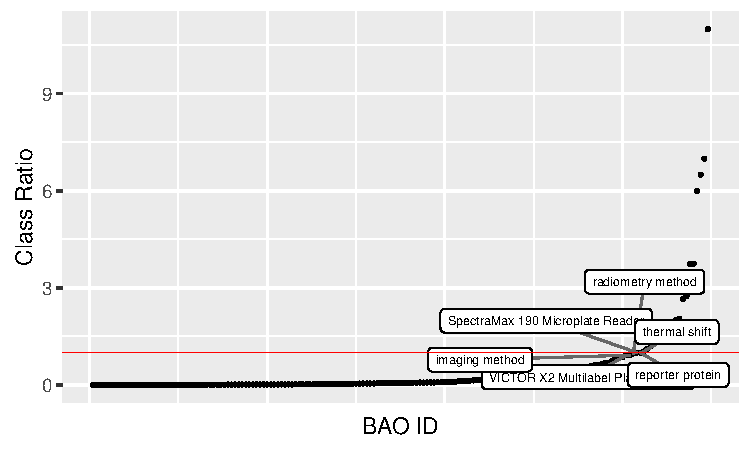
\includegraphics[width=0.9\textwidth]{img-nbclassratio-v2}
\end{frame}

\begin{frame}
  \frametitle{Training Set Performance}
  \begin{itemize}
  \item Matthews Correlation Coefficient
  \end{itemize}
\end{frame}

%%%% Ending slides
\begin{frame}
  \frametitle{Pitfalls}
  \centering{
    \parbox{0.75\textwidth}{
      \textit{\color{red}If sufficiently annotated, compound behavior can be 
        correlated to assay and biology characteristics}}
}
\vskip 1em
  \begin{itemize}
  \item A very abstract, possibly lossy, view of the effect of compounds on biology
  \item Depends on correct and meaningful annotations
  \item Annotations terms are context dependent, but this may not be considered when annotating a dataset
  \item BAO terms exhibit hierarchical relationships and ignoring them
    is simplistic
  \end{itemize}
\end{frame}

\begin{frame}
  \frametitle{Acknowledgements}
  \begin{itemize}
  \item Qiong Cheng (U. Miami)
  \item Stephan Sch\"{u}rer (U. Miami)  
  \end{itemize}
\end{frame}
\end{document}
